\documentclass[]{article}


\usepackage{float}
\usepackage[italian]{babel}

% Set page size and margins
% Replace `letterpaper' with`a4paper' for UK/EU standard size
\usepackage[letterpaper,top=3cm,bottom=3cm,left=3cm,right=3cm,marginparwidth=1.75cm]{geometry}

% Useful packages
\usepackage{amsmath}
\usepackage{graphicx}
\usepackage[colorlinks=true, allcolors=blue]{hyperref}


\title{SMSecure - Documentazione}
\author{Samuele Russo   matr.0512113317}


\begin{document}
\maketitle

\newpage

\tableofcontents

\newpage


\section{Introduzione}

    L'aumento esponenziale dell'utilizzo di dispositivi mobili ha reso gli SMS uno dei principali canali di comunicazione. Tuttavia, insieme a questa crescita, si è verificato un forte incremento del numero di spam SMS; ovvero messaggi caratterizzati da contenuti promozionali non richiesti, pubblicità ingannevoli o addirittura truffe; compromettendo l'efficienza e la sicurezza delle comunicazioni personali e professionali.


    \subsection{Obiettivi}

        Il mio progetto di FIA, prima esperienza personale in questo ambito, si propone di sviluppare un filtro anti-spam per migliorare l'esperienza degli utenti nel gestire i propri SMS. Ho deciso tale tematica perchè relativamente semplice, e di conseguenza in grado di farmi apprendere le basi del ML.

        Gli obiettivi principali includono:
        \begin{itemize}
            \item l'analisi approfondita di grandi quantità di SMS        estrapolati da un dataset.
            \item l'identificazione di feature associate ai               messaggi indesiderati.
            \item l'implementazione di un modello di apprendimento in grado di classificare in modo affidabile messagi spam e legittimi.
        \end{itemize}

    \subsection{Specifica PEAS}
        \begin{itemize}
            \item Performance (misure di prestazione adottate per valutare l’operato di un agente), nel mio caso verrà valutata la precisione di classificazione, ovvero il rapporto tra il numero di messaggi spam correttamente identificati e il totale dei messaggi classificati. Inoltre, sarà anche considerato il tasso di falsi positivi, ovvero messaggi legittimi che vengono erroneamente etichettati come spam.
            \item Environment (elementi che formano l’ambiente), nel mio caso sarà costituito dal flusso di messaggi ricevuti. 'vedi specifiche in 1.3'
            \item Actuators (attuatori disponibili all’agente per intraprendere le azioni), nel mio caso sarà la capacità del sistema di etichettare i messaggi in arrivo come spam o non spam.
            \item Sensors (sensori attraverso i quali l'agente riceve gli input percettivi), nel mio caso l'agente va ad acquisire i dati utili per classificare un messaggio, incluso il contenuto del messaggio, ma anche eventuali feature costruite (numero di parole ecc.)
        \end{itemize}

        \subsection{Caratteristiche dell'ambiente}
            L'ambiente è:
            \begin{itemize}
                \item Parzialmente osservabile, in quanto non si ha accesso alle informazioni del mittente.
                \item Stocastico, infatti i messaggi inviati dagli utenti sono influenzati da fattori non prevedibili.
                \item Singolo agente, in quanto c'è un solo questo filtro anti-spam in un client di messaggistica.
                \item Dinamico, difatti potrebbero venire a crearsi nuovi schemi di messaggi spam.
                \item Discreto, in quanto non sono presenti variabili continue (difatti una variabile continua potrebbe essere la frequenza di invio di un determinato mittente, ma io non ho trovato tale informazioni).
                \item Sequenziale, difatti il filtro anti-spam verrà pienamente influenzato dalle esperienze passate, per andare a prendere delle decisioni.
            \end{itemize}

        \newpage
        \subsection{Analisi del problema}
            Questo semplice progetto mira quindi a costruire un filtro anti-spam sms, si tratta quindi di un problema di Machine Learning, più nello specifico di un problema di apprendimento supervisionato, nonchè di classificazione. Nelle successive sezioni vado a descrivere tutte le problematiche che ho affrontato: dalla scelta dei dati, fino al deploy del modello.\\
            Per quanto riguarda le tecnologie che ho utilizzato per lo sviluppo del progetto, abbiamo:
            \begin{itemize}
                \item Python (in dettaglio le librerie per ML, come sickitLearn, Pandas,  ecc.),
                \item JupyterNotebook all'interno dell'IDE PyCharm
                \item GitHub per il versionamento
                \item Per quanto riguarda documentazione e presentazione overleaf (editor latex) e powerpoint rispettivamente.
            \end{itemize}
\newpage
\section{Data Understanding}
    Tale fase è composta da più punti:
    \begin{itemize}
        \item Acquisizione dei dati (scelta del dataset)
        \item Esplorazione dei dati
        \item Analisi della qualità dei dati
    \end{itemize}
    \subsection{Acquisizione dei dati}
        L'acquisizione dei dati è il processo di raccolta, ed organizzazione dei dati necessari per andare a creare un modello di ML. Con gli obiettivi chiari e definiti, sono andato alla ricerca di un dataset sul web, fino a trovarne uno molto interessante su Kaggle; una piattaforma, nonchè comunità online di data science. \\

        \begin{figure}[H]
            \centering
            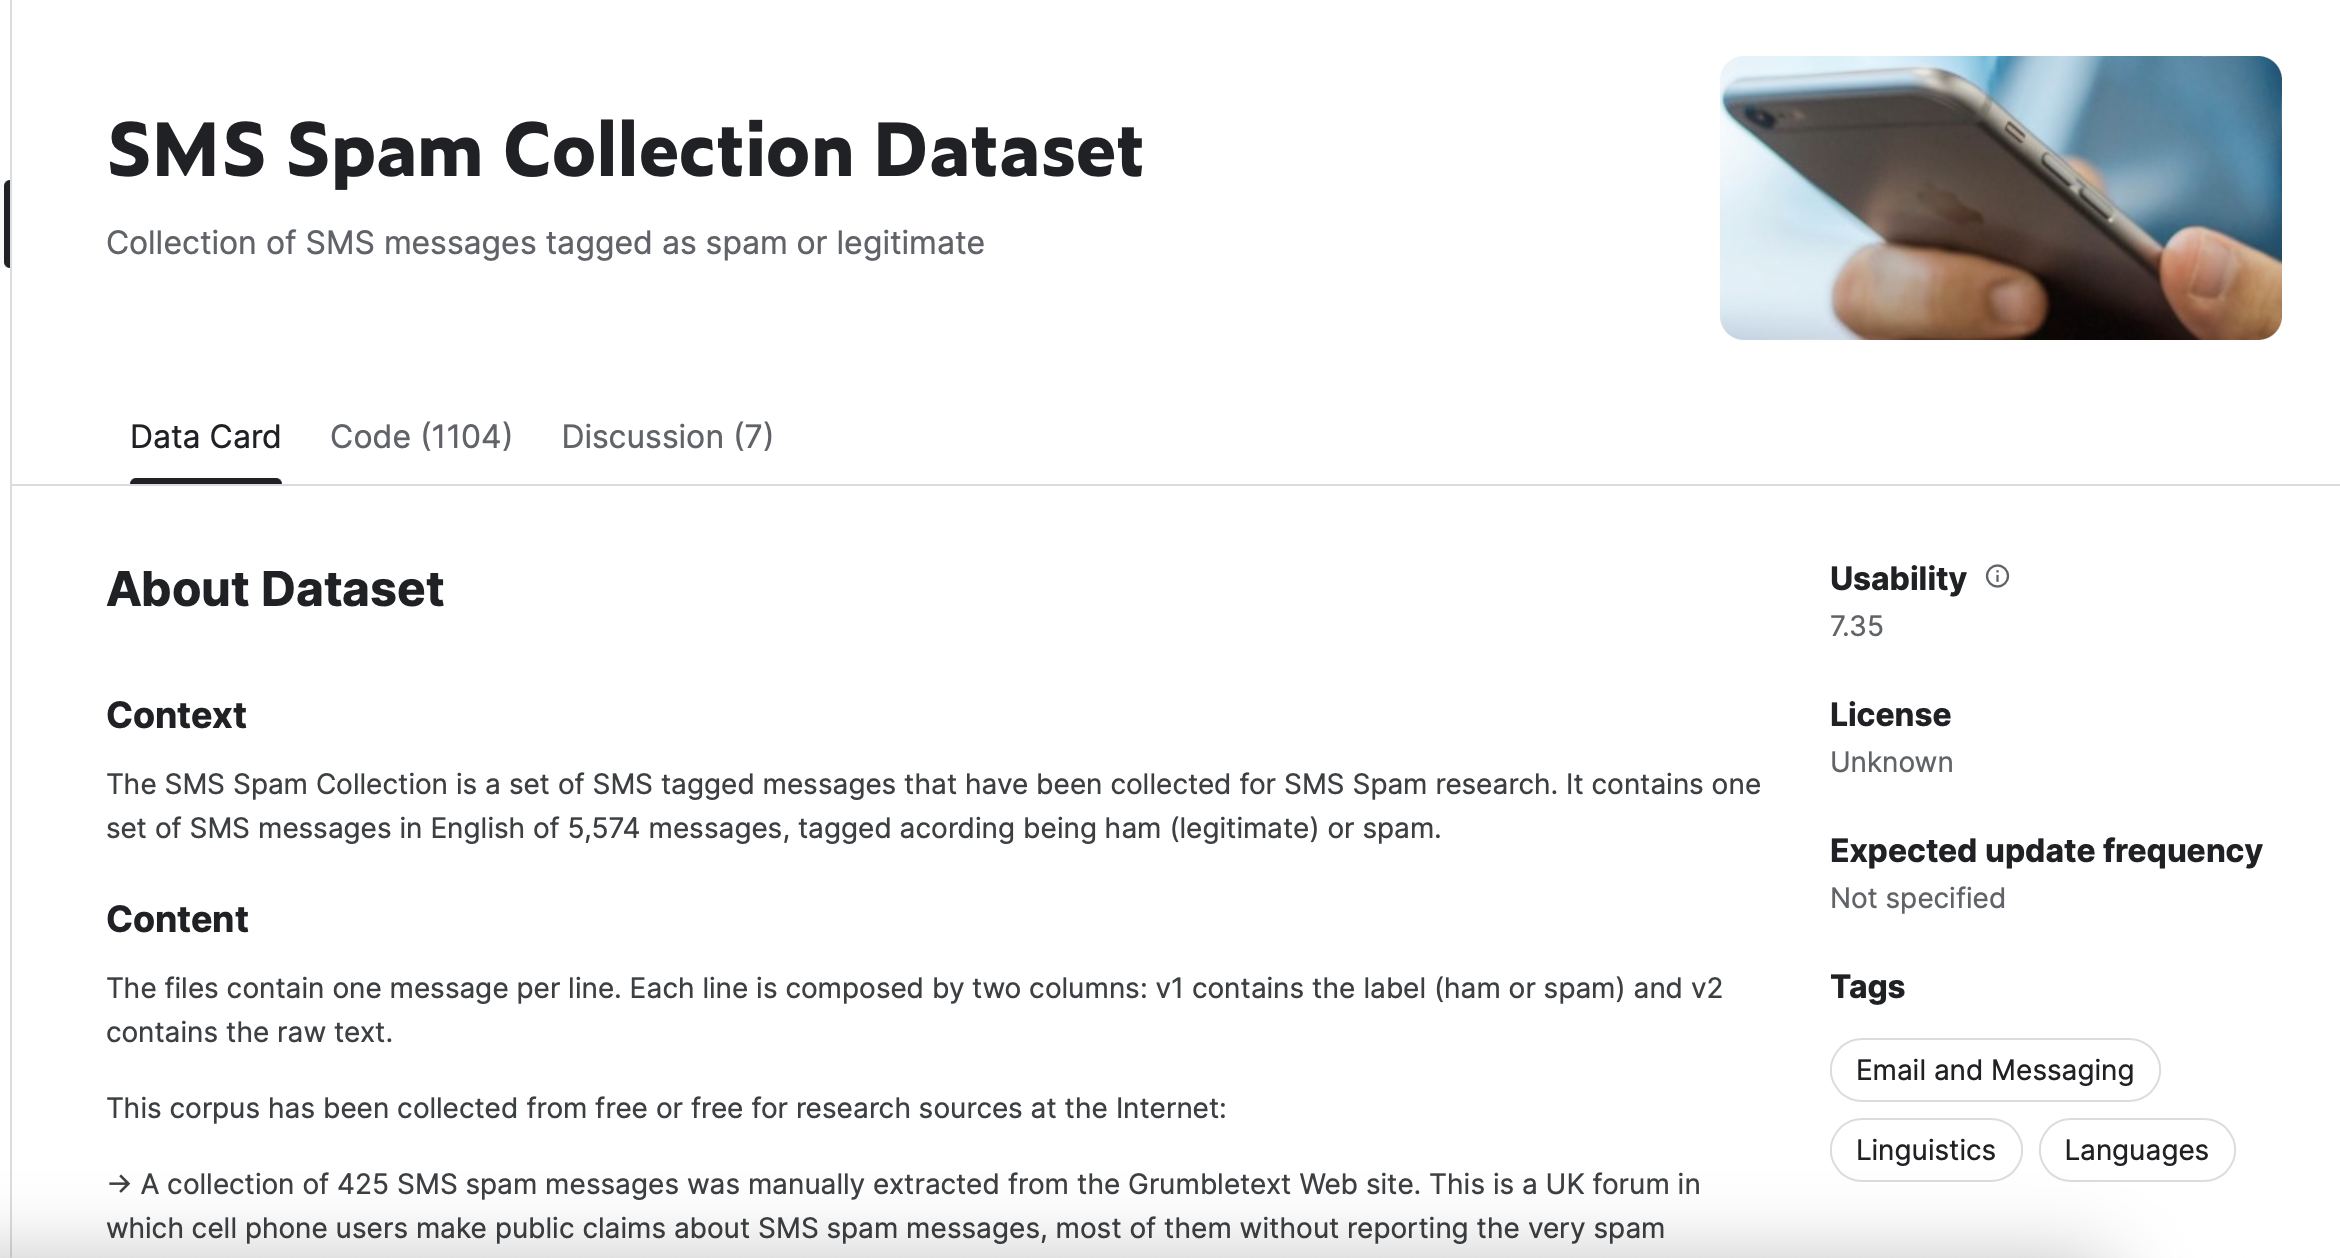
\includegraphics[width=1\linewidth]{images/kaggleDataset.png}
            \caption{Dataset su kaggle.com}
            \label{fig:enter-label}
        \end{figure}

    \subsection{Esplorazione dei dati}
        Il dataset in esame "SMS Spam Collection" è un insieme di messaggi SMS etichettati. Comprende 5.574 messaggi in inglese, suddivisi tra "ham" (legittimi) e "spam". Ogni messaggio è rappresentato da una riga con due colonne: una contiene l'etichetta (ham o spam) ed una contiene il testo grezzo dell'SMS. In questa fase vado ad analizzare, o meglio esplorare più nel dettaglio i dati per comprenderli e per scoprire informazioni rilevanti, tendenze, o relazioni. \\
        Quindi sono andato a fare una prima panoramica del dataset, andando a conteggiare quanti sample per ogni classe (ham/spam) fossero presenti, i nomi delle colonne, per poi passare alla vera esplorazione dei dati, volta quindi a trovare informazioni maggiormente rilevanti.\\
        Per un messaggio di testo è molto interessante andare ad osservare la sua lunghezza, il numero di parole al suo interno ed anche il numero di frasi. Non disponendo di tali feature sono andato a ricavarle, andando ad anticipare la \textbf{feature construction} della fase di Data Preparation.\\
        Per andare a ricavare queste feature dal testo ho utilizzato delle funzioni disponibili nella libreria nltk (conteggio parole e frasi), nonchè la funzione len() per calcolare il numero di caratteri. \\
        Per visualizzare eventuali trend e relazioni tra le varie feature, ho utilizzato alcuni grafici del libreria seaborn. Iniziamo ad analizzare i risultati ottenuti, partendo dal numero di caratteri.

        \begin{figure}[H]
            \centering
            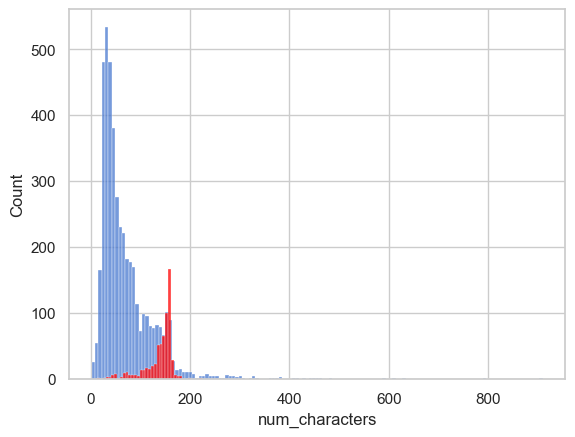
\includegraphics[width=0.6\linewidth]{images/num_char.png}
            \caption{numero di caratteri nei messaggi}
            \label{fig:enter-label}
        \end{figure}

        È da notare che in rosso sono rappresentati gli SMS spam, mentre in blu quelli ham. Sull'asse y la varibaile count indica il numero di volte in cui un determinato messaggio ha un certo numero di caratteri. Compreso ciò dal grafico è subito possibile notare che i messaggi spam hanno un numero di caratteri mediamente maggiore dei messaggi ham. \\
        Vediamo ora cosa emerge dal grafico che rappresenta il numero di parole.\\

        \begin{figure}[H]
            \centering
            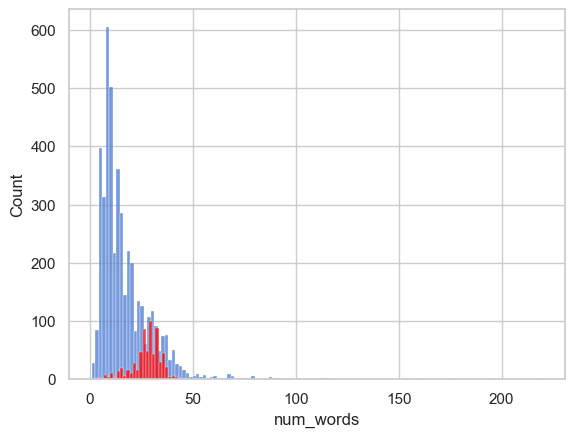
\includegraphics[width=0.6\linewidth]{images/num_words.png}
            \caption{numero di parole nei messaggi}
            \label{fig:enter-label}
        \end{figure}

        Si nota che vale lo stesso per il numero delle parole, difatti a rigor di logica il numero di parole è fortemente correlato al numero di caratteri, e quindi sarà lo stesso anche per il numero di frasi. Per vedere ancora più chiaramente tale correlazioni sono andato ad utilizzare un grafico riassuntivo, un pairplot.In tale tipo di grafico, ogni variabile numerica presente nel dataset viene confrontata con tutte le altre variabili numeriche tramite dei grafici a dispersione, che quindi consentono di visualizzare e individuare ancora meglio eventuali relazioni o tendenze.

        \begin{figure}[H]
            \centering
            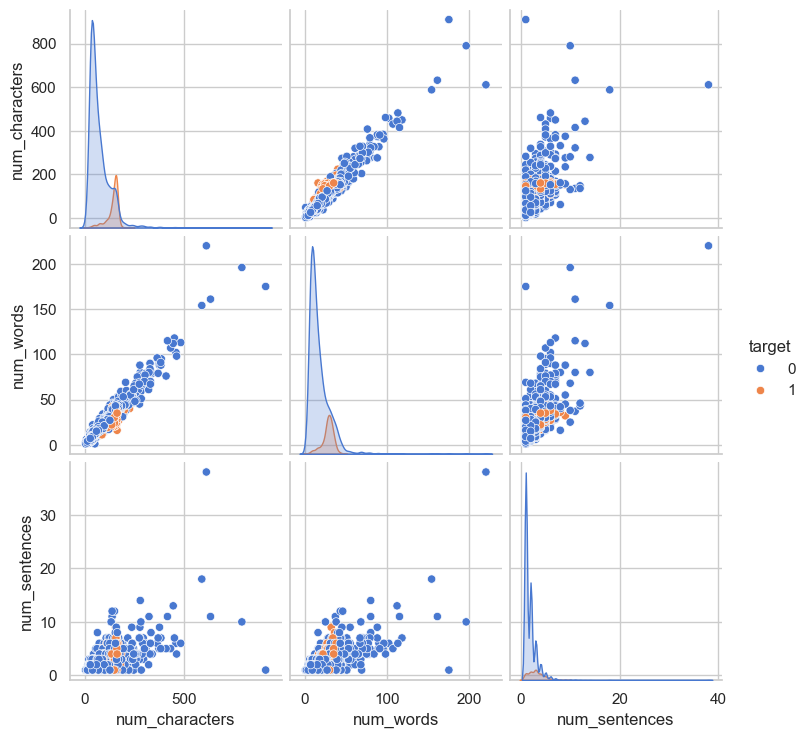
\includegraphics[width=1\linewidth]{images/sns_riassuntivo.png}
            \caption{pairplot riassuntivo}
            \label{fig:enter-label}
        \end{figure}

        Dal grafico emerge, ancora una volta, che:
        \begin{itemize}
        \item gli sms spam hanno in media un numero di caratteri maggiore
        \item gli sms spam hanno in media un numero di parole maggiore
        \item il numero di frasi è invece molto molto simile
    \end{itemize}

     Infine, per calcolare la correlazione tra le variabili, possiamo usare un'ulteriore strumento: la heatmap, una mappa che utilizza colori per visualizzare i valori dei coefficienti di correlazione tra le diverse coppie di variabili nel dataset, consentendo di individuare facilmente relazioni tra di esse. Le celle più scure o più chiare indicano correlazioni più forti o più deboli, rispettivamente. Le variabili sono fortemente correlate tra loro se hanno valori vicini a 1 o -1, mentre hanno una bassa correlazione se hanno valori vicini a 0.

     \begin{figure}[H]
            \centering
            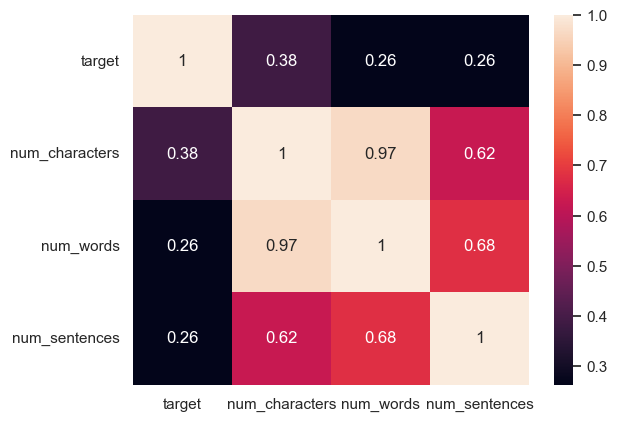
\includegraphics[width=1\linewidth]{images/matrice_corr.png}
            \caption{HeatMap}
            \label{fig:enter-label}
    \end{figure}

    E qui possiamo finalmente visualizzare l'effettiva correlazione tra le variabili. Si può notare con estrema facilità l'altissima correlazione tra il numero di caratteri e il numero di parole, cosa che è un pò meno marcata con il numero di frasi.\\
   Un'altra cosa davvero molto interessante è andare a visualizzare quali paroli sono più o meno frequenti nelle rispettive categoria di messaggi.